\documentclass[journal]{vgtc}                % final (journal style)
%\documentclass[review,journal]{vgtc}         % review (journal style)
%\documentclass[widereview]{vgtc}             % wide-spaced review
%\documentclass[preprint,journal]{vgtc}       % preprint (journal style)

%% Uncomment one of the lines above depending on where your paper is
%% in the conference process. ``review'' and ``widereview'' are for review
%% submission, ``preprint'' is for pre-publication, and the final version
%% doesn't use a specific qualifier.

%% Please use one of the ``review'' options in combination with the
%% assigned online id (see below) ONLY if your paper uses a double blind
%% review process. Some conferences, like IEEE Vis and InfoVis, have NOT
%% in the past.

%% Please note that the use of figures other than the optional teaser is not permitted on the first page
%% of the journal version.  Figures should begin on the second page and be
%% in CMYK or Grey scale format, otherwise, colour shifting may occur
%% during the printing process.  Papers submitted with figures other than the optional teaser on the
%% first page will be refused. Also, the teaser figure should only have the
%% width of the abstract as the template enforces it.

%% These few lines make a distinction between latex and pdflatex calls and they
%% bring in essential packages for graphics and font handling.
%% Note that due to the \DeclareGraphicsExtensions{} call it is no longer necessary
%% to provide the the path and extension of a graphics file:
%% 
\includegraphics{diamondrule} is completely sufficient.
%%
\ifpdf%                                % if we use pdflatex
  \pdfoutput=1\relax                   % create PDFs from pdfLaTeX
  \pdfcompresslevel=9                  % PDF Compression
  \pdfoptionpdfminorversion=7          % create PDF 1.7
  \ExecuteOptions{pdftex}
  \usepackage{graphicx}                % allow us to embed graphics files
  \DeclareGraphicsExtensions{.pdf,.png,.jpg,.jpeg} % for pdflatex we expect .pdf, .png, or .jpg files
\else%                                 % else we use pure latex
  \ExecuteOptions{dvips}
  \usepackage{graphicx}                % allow us to embed graphics files
  \DeclareGraphicsExtensions{.eps}     % for pure latex we expect eps files
\fi%

%% it is recomended to use ``\autoref{sec:bla}'' instead of ``Fig.~\ref{sec:bla}''
\graphicspath{{gfx/}{./}} % where to search for the images

\usepackage{microtype}                 % use micro-typography (slightly more compact, better to read)
\PassOptionsToPackage{warn}{textcomp}  % to address font issues with \textrightarrow
\usepackage{textcomp}                  % use better special symbols
\usepackage{mathptmx}                  % use matching math font
\usepackage{times}                     % we use Times as the main font
\renewcommand*\ttdefault{txtt}         % a nicer typewriter font
\usepackage{cite}                      % needed to automatically sort the references
\usepackage{tabu}                      % only used for the table example
\usepackage{booktabs}                  % only used for the table example
\usepackage{makecell}
\usepackage{multirow}

%% We encourage the use of mathptmx for consistent usage of times font
%% throughout the proceedings. However, if you encounter conflicts
%% with other math-related packages, you may want to disable it.

%% In preprint mode you may define your own headline.
%\preprinttext{To appear in IEEE Transactions on Visualization and Computer Graphics.}

%% If you are submitting a paper to a conference for review with a double
%% blind reviewing process, please replace the value ``0'' below with your
%% OnlineID. Otherwise, you may safely leave it at ``0''.
\onlineid{0}

%% declare the category of your paper, only shown in review mode
\vgtccategory{Research}
%% please declare the paper type of your paper to help reviewers, only shown in review mode
%% choices:
%% * algorithm/technique
%% * application/design study
%% * evaluation
%% * system
%% * theory/model
\vgtcpapertype{theory/model}

%% Paper title.
\title{Computing Graphical Perception}

%% This is how authors are specified in the journal style

%% indicate IEEE Member or Student Member in form indicated below
\author{Daniel Haehn, \textit{Member, IEEE}, James Tompkin, and Hanspeter Pfister}
\authorfooter{
%% insert punctuation at end of each item
\item Daniel Haehn, and Hanspeter Pfister are with the Paulson School of Engineering and Applied Sciences at Harvard University. \\
E-mail: \{haehn,pfister\}@seas.harvard.edu.
%
\item James Tompkin is with the Thomas J. Watson Sr. Center for Information Technology at Brown University. \\E-mail: james\_tompkin@brown.edu.
}

%other entries to be set up for journal
\shortauthortitle{Haehn \MakeLowercase{\textit{et al.}}: Computing Graphical Perception}
%\shortauthortitle{Firstauthor \MakeLowercase{\textit{et al.}}: Paper Title}

%% Abstract section.
\abstract{TODO%
} % end of abstract

%% Keywords that describe your work. Will show as 'Index Terms' in journal
%% please capitalize first letter and insert punctuation after last keyword
\keywords{Machine Perception, Deep Learning}

%% ACM Computing Classification System (CCS). 
%% See <http://www.acm.org/class/1998/> for details.
%% The ``\CCScat'' command takes four arguments.

%\CCScatlist{ % not used in journal version
% \CCScat{K.6.1}{Management of Computing and Information Systems}%
%{Project and People Management}{Life Cycle};
% \CCScat{K.7.m}{The Computing Profession}{Miscellaneous}{Ethics}
%}

%% Uncomment below to include a teaser figure.
\teaser{
  \centering
  \includegraphics[width=\linewidth]{teaser.pdf}
  \caption{\textbf{Computing Cleveland and McGill's Position-Angle Experiment using Convolutional Neural Networks.} We replicate the original experiment by asking visual cortex inspired machine learning classifiers to assess the relationship between values encoded in pie charts and bar charts. Similar to the findings of Clevenland and McGill~\cite{cleveland_mcgill}, our experiments show that CNNs predict more accurately when working with bar charts (mean squared error, MSE in green).}
	\label{fig:teaser}
}

%% Uncomment below to disable the manuscript note
%\renewcommand{\manuscriptnotetxt}{}

%% Copyright space is enabled by default as required by guidelines.
%% It is disabled by the 'review' option or via the following command:
% \nocopyrightspace

\vgtcinsertpkg

%%%%%%%%%%%%%%%%%%%%%%%%%%%%%%%%%%%%%%%%%%%%%%%%%%%%%%%%%%%%%%%%
%%%%%%%%%%%%%%%%%%%%%% START OF THE PAPER %%%%%%%%%%%%%%%%%%%%%%
%%%%%%%%%%%%%%%%%%%%%%%%%%%%%%%%%%%%%%%%%%%%%%%%%%%%%%%%%%%%%%%%%

\begin{document}

%% The ``\maketitle'' command must be the first command after the
%% ``\begin{document}'' command. It prepares and prints the title block.

%% the only exception to this rule is the \firstsection command

\firstsection{Introduction}

\maketitle

Artificial intelligence has taken the world of technology by storm. Deep multilayer neural networks are being successfully applied in a wide range of applications that are regularly outperforming humans in object recognition \cite{krizhevsky_imagenet2012, simonyan_very_deep2014,szegedy2015}. 
Originally inspired by neuroscientific discoveries, the recent advances in deep learning have been the direct results of engineering efforts, more specifically in convolutional neural networks (CNNs). 
While there has been significant advancement, this does not mean we understand what CNNs are doing and we are in fact treating them as blackboxes without detracting from their success \cite{goodfellow_book, deeplearning_blackbox2017}. 
Our current knowledge of biological vision suggests that modern machine learning models indeed mimic the underlying biology by abstracting the many details of biological neural networks \cite{yamins2016using, hassabis2017neuroscience}.

Despite tremendous research efforts and generating massive datasets, we are far from fully understanding biological vision. 
Similarly, we are constantly developing inventive features for deep artificial networks without truly understanding it in its entirety. As a result, a double discrepancy is observed. 
Advances in neuroscience can revolutionize machine learning by reverse-engineering neural circuits, yielding new classifiers which, in turn, can help process the massive biological data. 
There are many existing questions which must be answered in order to fill this gap of our understanding.

We focus on perception... experiments from cleveland mcgill..



%\emph{Can we leverage decades of visualization research to understand the way convolutional neural networks process data?}
%
%Information visualization has been an established research field for decades which has resulted in numerous insightful findings in regards to how human beings can best process information visually.
%Unpublished preliminary experiments have shown that data representations customized for the human eye also can improve the performance of an automatic classifier. 
%While the reasons for this are still unknown, specified research can most certainly advance the understanding of deep neural networks.

\subsection{Biological Vision}

\begin{figure}[t]
	  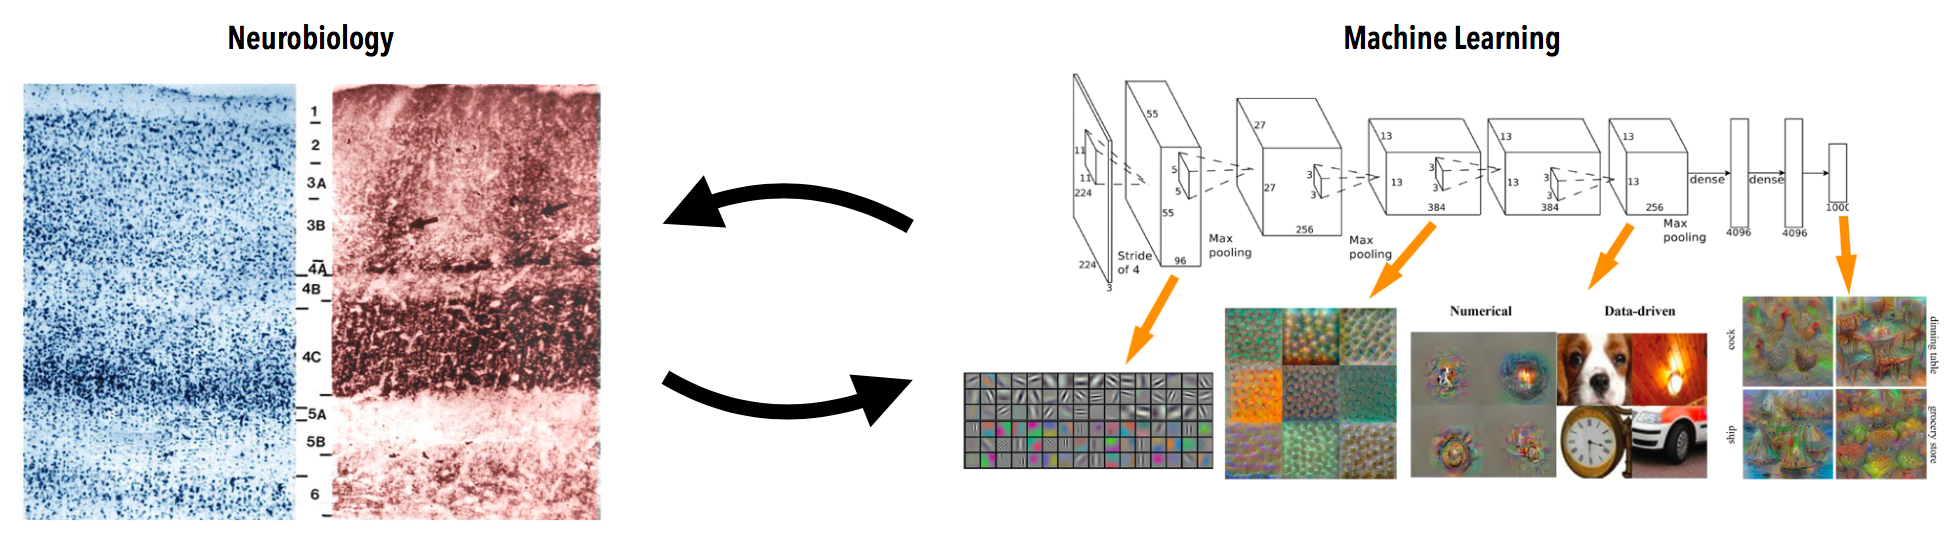
\includegraphics[width=\linewidth]{biology_vs_cnn.png}
  \caption{The Biological Vision (schematic)}
	\label{fig:vision}
\end{figure}

Biological vision is an extremely powerful system which allows humans the ability, and seemingly without effort, to recognize an enormous amount of distinct objects in the world. 
Object detection is extremely difficult and therefore is especially impressive as light intensities can change by levels of magnitude and contrast between foreground and background is so often low. 
In addition, the visual scene changes every time the human body or human eyes move. 
This visual system exhibits a very noisy structure but because it is organized by layers it has inspired the mathematical theory of multilayer neural networks. 
What is remarkable is that even though current machine learning models do not resemble the complexity of its biological pendant, they inherently generalize extremely well. 
Neural networks trained on one specific task can be used to perform detection or segmentation of, seemingly, unrelated objects with relatively minor retraining. 
The reported classification performance is superior to that of humans and the question in regards to their functionality opens an interesting research topic.


GOALS
...reduce the gap between neurobiology and data science to advance the understanding of visual cortex inspired machine learning

CONTRIBUTIONS

- experiments of cleveland mcgill with systematic parametrization and evaluation

- ranking like cleveland mcgill for machine perception?

- many other insights?

- framework





\section{Previous Work}

\textbf{Graphical Perception.} Cleveland and McGill~\cite{cleveland_mcgill} introduce the fundamental concept of \emph{graphical perception} and investigate how different visual attributes and encodings are perceivable by humans. They define \emph{elementary perceptual tasks} as mental-visual stimuli to understand encodings in visualizations. Based on these definitions, the authors propose and perform different experiments such as the \emph{position-angle} experiment which compares bar charts and pie charts, the \emph{position-length} experiment where users judge relations between encoded values in grouped and divided bar charts, and the \emph{bars-and-framed-rectangles} experiment to evaluate Weber's law. Heer and Bostock later reproduced the Cleveland-McGill experiments crowd-sourced on Mechanical Turk~\cite{HeerBostock2010} which lead to follow-up work from Harrison \textit{et al.}~\cite{harrison2013influencing} who replicated the experiments while observing emotional states. Both papers report similar results to Cleveland and McGill which increased our motivation to mimmick their pioneering work. Our experimental setup replicates the original setup of Cleveland and McGill - just instead of humans, we use convolutional neural networks due to the connection with the human visual system. While we focus on Cleveland and McGill's work from 1984, many other excellent articles from the last decades target low-level visual encoding~\cite{bertin1967semiologie,cleveland1985graphical,treisman1988feature, wilkinson2006grammar, carpendale2003considering,widgor_perception2007,munzner2015visualization}.

Interesting are also the rankings of correlation visualization using Weber's law~\cite{harrison2014_webers_law_rank}. This law defines the proportional relation between the initial distribution density and perceivable change. In this paper, we investigate with a simple experiment whether this holds for convolutional neural networks.
\\~\\
%\textbf{Comparing Visual Encodings.} Different visual encodings have advantages or disadvantages and the community does a great job comparing them. Higher-level comparisons include 2D versus 3D vector field and rendering studies~\cite{mckenzie_2d_3d,forsberg2009comparing_3d_vector,laidlaw_2d_vector,borkin2011arteries}, timeseries~\cite{herr2009timeseries} and scatterplots~\cite{tremmel1995visual,Wang_linegraph_vs_scatterplot}. Lower-level experiments target - besides others - open versus closed encodings~\cite{open_vs_closed_shapes}, and several evaluations of color space~\cite{ware1988color,rheingans1992color,Rogowitz2001_colormaps,kindlmann2002color}. While we investigate lower-level visual encodings in this work, we delay colorspace experiments for future work.

\textbf{Computational Visualization Understanding.}

Pineo \textit{et al.}~\cite{Pineo2012_computational_perception} create computational model of human vision based on neural networks and their experiments show that understanding visualization triggers neural activity in high-level areas of cognition. The authors suspect that this level of understanding is produced by low-level neurons performing elementary perceptional tasks. We are further investigating this suspision.
Other work tries to parse infographics by finding higher-level saliency models~\cite{bylinskii2016should}, or by extracting text or key visual elements~\cite{diagram_understanding,kembhavi2016diagram,zoya_text_visual_tags}. However, none of these works focus on computational understanding of lower-level building blocks of visualizations such as curvature, lengths, or position.
\\~\\
\textbf{Visual Cortex Inspired Machine Learning.} 
%Classifiers mimmicking the human visual system are a hot topic and many different architectures, models, and paradigms exist. Feed-forward neural networks 
The human visual cortex is an extremely powerful system which allows the ability, and seemingly without effort, to recognize an enormous amount of distinct objects in the world. This visual system is organized in layers and has inspired the theory of computational classifiers based on multilayer neural networks. Fukushima and Miyake developed the Neocognitron quantitative model~\cite{fukushima1982neocognitron} that ultimately led to the important work of Hinton, Bengio, and LeCun: \textit{deep neural networks}~\cite{lecun2015deep}, visual cortex inspired machine learning.
Nowadays, such classifiers exist with many different architectures. For this paper, we select the traditional \emph{LeNet-5}~\cite{lenet} which was designed to recognize hand-written digits, the VGG19~\cite{simonyan_very_deep2014} classifier with 16 convolutional layers, and the Xception~\cite{xception} classifier with 36 convolutional layers. Selecting these specific networks allows us to compare archtitectures with different depths.
%Object detection is extremely difficult and therefore is especially impressive as light intensities can change by levels of magnitude and contrast between foreground and background is so often low. 
%In addition, the visual scene changes every time the human body or human eyes move. 
%This visual system exhibits a very noisy structure but because it is organized by layers it has inspired the mathematical theory of multilayer neural networks. 

%In 1962 Hubel and Wiesel were the first to begin studying the visual cortex from the standpoint of a neuroscientist. Their experimental findings on cats and macaque monkeys suggested a hierarchy of cells with increasing complexity which was then later transferred to the hierarchical model of different layers. Twenty years later, this insight was translated to the Neocognitron quantitative model, by Fukushima and Miyake, which ultimately led to the important work of Hinton, Bengio, and LeCun in the 1980s. Their work on stochastic gradient descent approximation, and the availability of faster computer hardware then led to today’s deep learning networks. In the last decade, this field has exhibited rapid growth, constant evolution, and new applications in various domains.


%The reported classification performance is superior to that of humans and the question in regards to their functionality opens an interesting research topic.
%Visual cortex inspired machine learning classifiers exist with many different architectures. We select the traditional \emph{LeNet-5}~\cite{lenet} which was designed to recognize hand-written digits, the VGG19~\cite{simonyan_very_deep2014} classifier with 16 convolutional layers, and the Xception~\cite{xception} classifier with 36 convolutional layers. 
%
%What is remarkable is that even though current machine learning models do not resemble the complexity of its biological pendant, they inherently are able to generalize but only after learning thousands of examples. 
%Neural networks trained on one specific task can be used to perform detection or segmentation of, seemingly, unrelated objects with relatively minor retraining~\cite{transfer_learning}. 
%
%
%We think that the biological inspiration of modern convolutional neural networks yields the evaluation of principles of human perception with computers.
%
%
%MLP, LeNet, VGG, ImageNet, XCeption, ResNets etc and work from THomas Serre
%
%
%- https://link.springer.com/chapter/10.1007/978-3-642-14600-8_46
%
%- https://github.com/tidyverse/ggplot2/wiki/Recommended-Reading
%
%- last year's VADL workshop: https://vadl2017.github.io/




\section{Experimental Setup}

The experiments shown in this paper are either supervised regression or classification tasks. We formulate any estimation of quantities (e.g. angles, positions, lengths etc.) as a regression problem between $0$ and $1$. The output indicates the percentage in regards to the degrees of freedom of the individual experiment. If the experiment involves a choice, we formulate it as a classification problem.

\subsection{Measures}

\textbf{Accuracy.} We use the same metric as Cleveland and McGill to measure accuracy.
\begin{equation}
	\log_2( | \textnormal{predicted percent} - \textnormal{true percent} | + .125)
\end{equation}
\\~\\
\noindent{\textbf{Confidence Intervals.}} We follow the notion of Cleveland and McGill to compute the confidence intervals.
\\~\\
\noindent{\textbf{Efficiency.}} We use the convergence rate based on the decrease of loss per training epoch as an indicator for the efficiency of the classifier in combination with a visual encoding. For regression tasks the loss is defined as mean squared error (MSE) and for classification tasks the loss is categorical cross-entropy.

\subsection{Classifiers}

Our classifiers are built upon a multilayer perceptron (MLP) which is a feedforward artificial neural network. We combine this MLP with different convolutional neural networks (CNNs) for preprocessing and feature generation. These include the traditional LeNet trained from scratch, as well as VGG19 and Xception trained using ImageNet.
\\~\\
\noindent{\textbf{Multilayer Perceptron.}} The multilayer perceptron in this paper has $256$ neurons which are activated as rectified linear units~(Fig.~\ref{fig:classifiers}). We then add a dropout layer to prevent overfitting and compute linear regression or classification (softmax).
\\~\\
\noindent{\textbf{Convolutional Neural Networks.}} We use CNNs to generate additional features as input to the MLP. We train the \emph{LeNet} classifier with tune it specifically towards each visualization. For \emph{VGG19} and \emph{Xception}, we generate features using previously trained weights on ImageNet.
\\~\\
\noindent{\textbf{Optimization.}} All networks are optimized using stochastic gradient descent with Nesterov momentum using fixed parameters (Table \ref{tab:parameters}). We train for $1000$ epochs but stop early if the loss does not decrease for ten epochs.
\\~\\
\noindent{\textbf{Environment.}} We run all experiments on an NVIDIA DGX1 machine with Tesla V100 graphical processing units. We use the KERAS framework with tensorflow.

\begin{table}[t]
\centering
\caption{We use different feature generators as input to a multilayer perceptron which performs linear regression or the classification task. This yields different sets of trainable parameters. We also train the MLP directly on the visualizations without any additional feature generation.}
\resizebox{\linewidth}{!}{
\begin{tabular}{lrl}
%	\toprule
%	\makecell{Classifier} & \makecell{Convolutional\\Layers} & \makecell{Trainable\\Parameters} \\
%	\midrule
%	MLP & $0$ & $2,560,513$ \\
%	\emph{LeNet} + MLP & $2$ & $8,026,083$ \\
%	\emph{VGG19} + MLP & $16$ & $21,204,545$ \\
%	\emph{Xception} + MLP & $36$ & $25,580,585$ \\
%	\bottomrule
	\toprule
	Classifier & \makecell{Trainable\\Parameters} & Optimization \\
	\midrule
	MLP & $2,560,513$ & SGD (Nesterov momentum)\\
	\emph{LeNet} + MLP & $8,026,083$ & Learning rate: $0.0001$\\
	\emph{VGG19} + MLP & $21,204,545$ & Momentum: $0.9$ \\
	\emph{Xception} + MLP & $25,580,585$ & \makecell[tl]{Batchsize: 32\\Epochs: $1000$ (Early Stopping)}\\
	\bottomrule
\end{tabular}
}
\label{tab:parameters}
\vspace{-4mm}
\end{table}

\begin{figure}[t]
	\centering
	  \includegraphics[width=.8\linewidth]{classifiers.pdf}
  \caption{The multilayer perceptron (MLP) in our experiments has 256 neurons which are activated as rectified linear units (ReLU). We use Dropout regularization to prevent overfitting. We learn categorical and unordered dependent variables using the softmax function and perform linear regression for continuous variables. The MLP can learn the visualizations directly but we also learn features generated by LeNet (2 conv. layers, filter size $5\time5$), VGG19 trained on ImageNet (16 conv. layers, filter size $3\times3$), or Xception trained on ImageNet (36 conv. layers, filter size $3\times3$) to increase the number of trainable parameters.}
	\label{fig:classifiers}
\end{figure}

\subsection{Data}

We create all visualizations as parametrized rasterized images without interpolation. The number of parameters differs per experiment as summarized in Table~\ref{tab:encoding_parameters} and section~\ref{sec:parametrizations}. We add subtle random noise ($0.05$) to each pixel to introduce additional variation.
\\~\\
\noindent\textbf{Training/Validation/Test Splits.} We specify the size of each split set as follows: 60,000 training images, 20,000 validation images, and 20,000 test images. We then randomly add parameterized visualizations to the sets while guaranteeing that each set is disjunct from each other in terms of encoded variables. This eliminates leakage during training and evaluation. We also scale each set independently: images to the range of $-.5$ to $.5$ and labels to the range of $0.0$ to $1.0$. 
\\~\\
\noindent\textbf{Cross-classifier variability.} We also evaluate classifiers previously trained with one visualization on the same type of visualizations with different parameters by decreasing and increasing the variability of the generated images.

\section{Elementary Perceptual Tasks}

Cleveland and McGill describe the mapping of graphical elements to quantitative variables as \emph{elementary perceptual tasks} and introduce a list of ten different encodings in their paper~\cite{cleveland_mcgill}. We create visualizations of these tasks as rasterized images (Fig.~\ref{fig:elementary_perceptual_tasks}).

\subsection{Parametrizations}
\label{sec:parametrizations}
We generate multiple parameterizations for each elementary perceptual task (Fig.~\ref{fig:elementary_perceptual_tasks}) and sequentially increase the number of parameters. For instance, for \emph{position non-aligned scale} we first only vary the origin of the coordinate system which yields just 10 different parameters. We then include translation along the y-axis with a significant increase in variability. We then also add x-movement and a variable spot size. This results in more complex datasets depending on the variability setting. Table~\ref{tab:encoding_parameters} shows the different settings. It is important to consider this variability when evaluating different classifiers with individual trainable parameters (Table~\ref{tab:parameters}).

\begin{figure}[t]
	  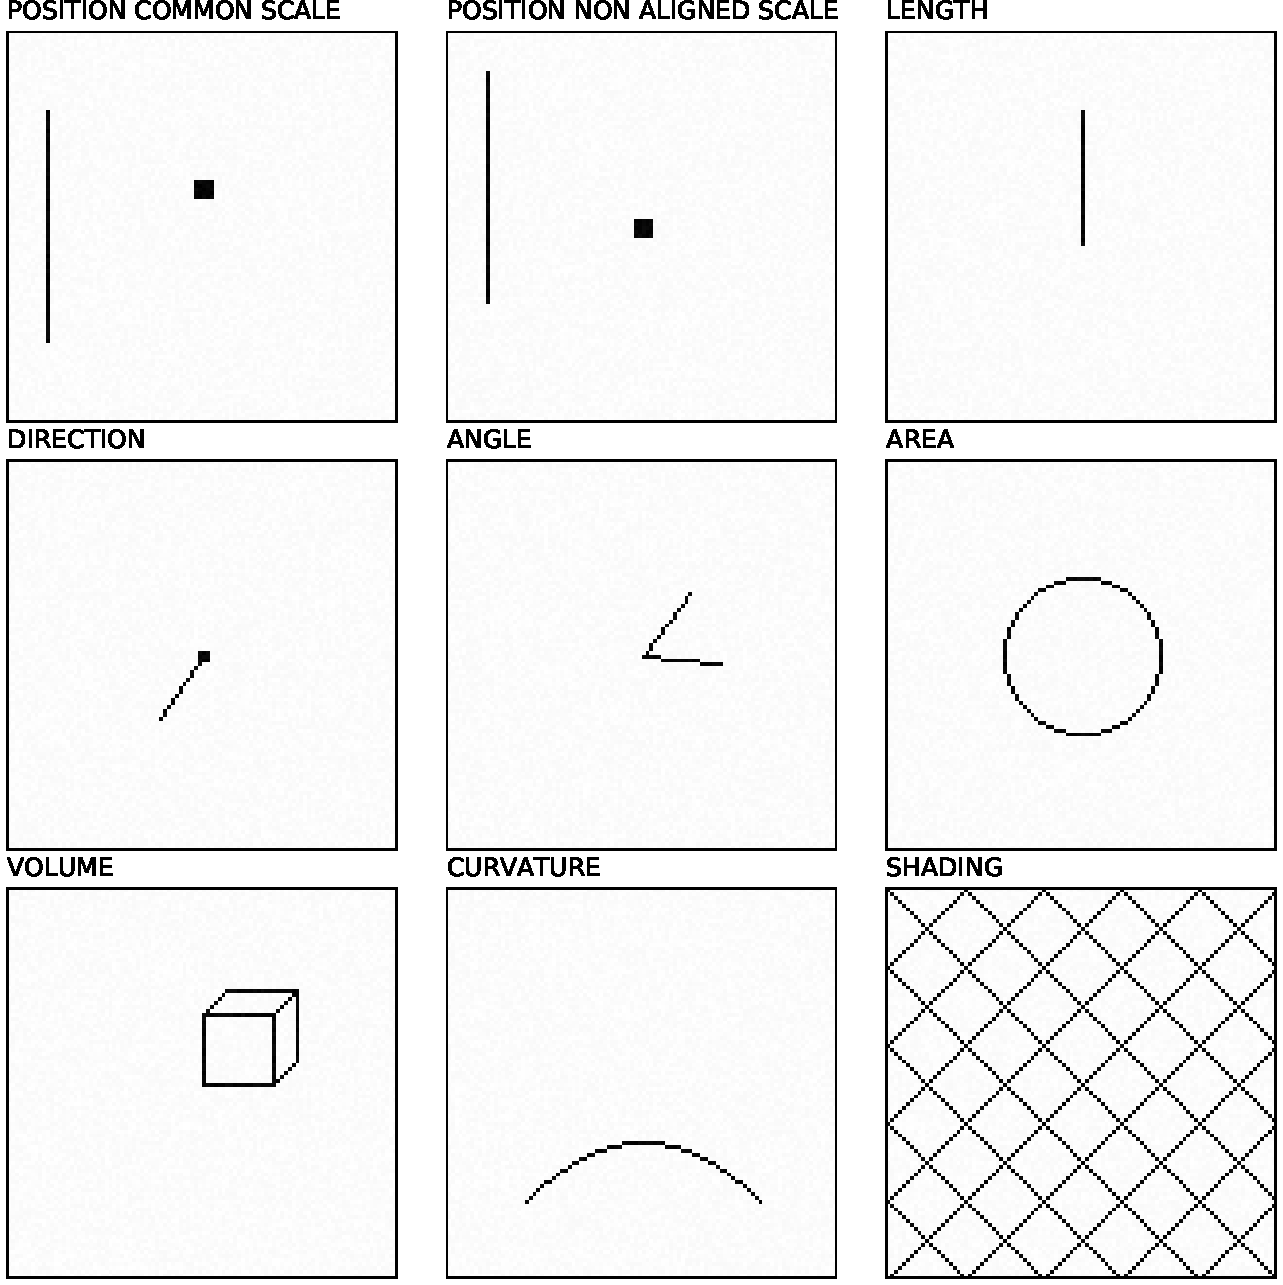
\includegraphics[width=\linewidth]{figure1_overview.pdf}
  \caption{\textbf{Elementary Perceptual Tasks.} Rasterized visualizations of the elementary perceptual tasks as defined by Cleveland and McGill~\cite{cleveland_mcgill} (color saturation excluded). We vary the parameters of each perceptual task and then assess the interpretability of feed-forward neural networks.}
	\label{fig:elementary_perceptual_tasks}
\end{figure}

\begin{table}[t]
\centering
\caption{\textbf{Variability of Elementary Perceptual Tasks.} We sequentially increase the number of parameters for every visual encoding of the elementary perceptual tasks. This introduces variability and increasingly more complex datasets.}
\resizebox{\linewidth}{!}{
\begin{tabular}{llr}
%	\toprule
%	\makecell{Classifier} & \makecell{Convolutional\\Layers} & \makecell{Trainable\\Parameters} \\
%	\midrule
%	MLP & $0$ & $2,560,513$ \\
%	\emph{LeNet} + MLP & $2$ & $8,026,083$ \\
%	\emph{VGG19} + MLP & $16$ & $21,204,545$ \\
%	\emph{Xception} + MLP & $36$ & $25,580,585$ \\
%	\bottomrule
	\toprule
	Elementary Perceptual Task & Variability & Parameters\\
	\midrule
	\makecell[tl]{\emph{Position Common Scale}} & \makecell[tl]{Position Y\\+ Position X \\+ Spot Size \\} & \makecell[tr]{ $60$ \\ $3600$ \\ $21600$}\\

	\midrule
	\makecell[tl]{\emph{Position Non-Aligned Scale}} & \makecell[tl]{Origin\\+ Position Y\\+ Position X \\+ Spot Size \\} & \makecell[tr]{ $10$ \\$600$ \\ $36000$ \\ $216000$}\\

	\midrule
	\makecell[tl]{\emph{Length}} & \makecell[tl]{Length\\+ Position Y \\+ Position X \\+ Width} & \makecell[tr]{ $60$ \\ $2400$ \\ $144000$\\$864000$}\\

	\midrule
	\makecell[tl]{\emph{Direction}} & \makecell[tl]{Angle\\+ Position Y \\+ Position X} & \makecell[tr]{ $360$ \\ $21600$ \\ $1296000$}\\

	\midrule
	\makecell[tl]{\emph{Angle}} & \makecell[tl]{Angle\\+ Position Y \\+ Position X} & \makecell[tr]{ $90$ \\ $5400$ \\ $324000$}\\

	\midrule
	\makecell[tl]{\emph{Area}} & \makecell[tl]{Radius\\+ Position Y \\+ Position X} & \makecell[tr]{ $40$ \\ $800$ \\ $16000$}\\

	\midrule
	\makecell[tl]{\emph{Volume}} & \makecell[tl]{Cube Sidelength\\+ Position Y \\+ Position X} & \makecell[tr]{ $20$ \\ $400$ \\ $8000$}\\
	
	\midrule
	\makecell[tl]{\emph{Curvature}} & \makecell[tl]{Midpoint Curvature\\+ Position Y \\+ Position X\\+ Width} & \makecell[tr]{ $80$ \\ $1600$ \\ $64000$ \\ $2560000$}\\	

	\midrule
	\makecell[tl]{\emph{Shading}} & \makecell[tl]{Density\\+ Position Y \\+ Position X} & \makecell[tr]{ $100$ \\ $1600$ \\ $2000$ \\ $40000$}\\	
	
	\bottomrule
\end{tabular}
}
\label{tab:encoding_parameters}
\end{table}

\subsection{Hypotheses}

We proposed four hypotheses entering the elementary perceptual task experiment:

\begin{itemize}
	\item \textbf{H1.1} \textbf{Visual cortex inspired classifiers are able to connect graphical elements to their quantitative variables.} While much simpler models than their biological pendant, convolutional neural networks are heavily influenced by our biological knowledge of the visual system. Such classifiers therefor follow the same principles as human perception.
	\item \textbf{H1.2} \textbf{Computed perceptual performance is dependent on classifier complexity.} We evaluate multiple classifiers with different numbers of trainable parameters. A more complex classifier (with higher number of parameters) will perform better on elementary perceptual tasks.
	\item \textbf{H1.3} \textbf{Some visual encodings are better than others for computations.} Cleveland and McGill order the elementary perceptual tasks by accuracy. We investigate whether this order is also relevant for computing graphical perception.
	\item \textbf{H1.4} \textbf{Classifiers trained on perceptual tasks can generalize to more or less complex variations of the same task.} Recent research suggests that convolutional neural networks generalize extremely well. While the underlying reasons are mainly yet unknown, this property allows them to perform on variations of a similar perceptual task.
\end{itemize}

\section{Position-Angle Experiment}

The position-angle experiment was originally performed by Cleveland and McGill to measure whether humans can better perceive quantities encoded as positions or as angles~\cite{cleveland_mcgill}. The actual experiment then compares pie charts versus bar charts since these map down to elementary position and angle judgement. We create rasterized images mimicking Cleveland and McGill's proposed encoding and investigate computational perception of our four classifiers.

\begin{figure}[t]
	  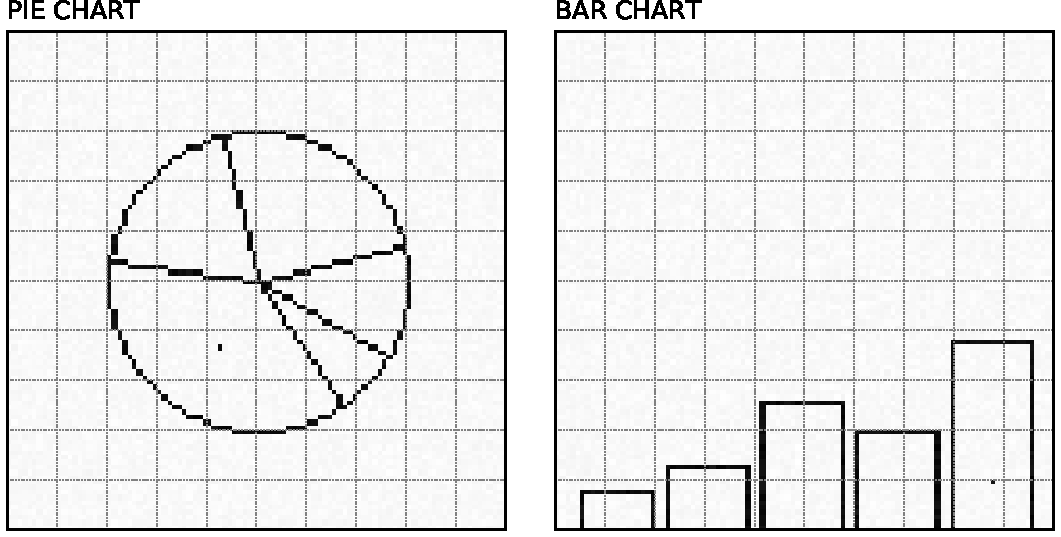
\includegraphics[width=\linewidth]{figure3_overview}
  \caption{\textbf{Position-Angle Experiment.} We create rasterized visualizations of pie charts and bar charts to follow Cleveland and McGill's position-angle experiment. The experimental task involves the judgement of different encoded values in comparison to the largest encoded values. The pie chart (left) and the bar chart (right) visualize the same data point. In their paper, Cleveland and McGill report less errors using bar charts.}
	\label{fig:position_angle_experiment}
\end{figure}

\subsection{Hypotheses}

We proposed four hypotheses entering the elementary perceptual task experiment:

\begin{itemize}
	\item \textbf{H2.1} \textbf{Computed perceptual performance is better using bar charts than pie charts.} Cleveland and McGill report that position judgements are almost twice as accurate as angle judgements. This renders bar charts superior to pie charts and should also be the case for convolutional neural networks.
	\item \textbf{H2.2} \textbf{Classifiers can learn position faster than angles.} We assume that understanding bar charts is easier than understanding pie charts. We suspect that our classifiers learn encodings of positions faster than of angles resulting in more efficient training and faster convergence.
\end{itemize}


\section{Position-Length Experiment}

This is the one where we estimate two selected bars compared to the longest one - very similar to the previous one but, not yet done. We basically test divided versus grouped barchart and we estimate one relation between two marked quanitities: what percent the smaller is of the larger.

There are five types: type 1-3 this is a position judgement along a common scale. (btw all classifiers seem to do that extremely well in the elementary tasks so we assume this will work well here too). Types 4-5 are length judgements and we know that the classifiers struggle with that quite a bit.

The setup from Cleveland McGill is first a classification task: which one is smaller? and then a regression task: how much smaller. So we have to see how to encode this.


\subsection{Hypotheses}

We proposed two hypotheses entering the elementary perceptual task experiment:

\begin{itemize}
	\item \textbf{H3.1} \textbf{Grouped bar charts are better computational perceivable than divided bar charts.} A grouped bar chart involves judging a position while a divided bar chart most likely (if not the bottom is looked at) requires length judgements. Classifiers are better at judging position than at judging length so grouped bar charts are easier to grasp in terms of computational perception.
	\item \textbf{H3.2} \textbf{not yet} Any ideas?
\end{itemize}


\begin{figure}[t]
	  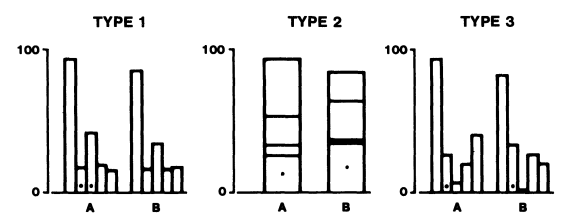
\includegraphics[width=\linewidth]{position_length_original1.png}
	  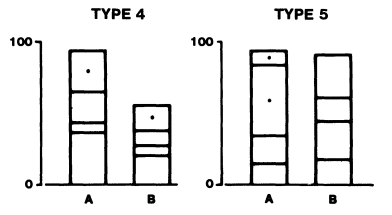
\includegraphics[width=\linewidth]{position_length_original2.png}
	  
  \caption{\textbf{Position-Length Experiment.} (Not yet) Rasterized versions of the graphs of Cleveland and McGill's position-length experiment. The perceptual task involves comparing. the two dot-marked quantities across five different visual encodings of either grouped or divided bar charts. We evaluate which type of bar chart performs better with our neural networks as a combined classification and regression problem. The first task is to select which of the marked quantities is smaller (classification) and the second task is to specify how much smaller it is (regression).}
	\label{fig:position_length_experiment}
\end{figure}

\section{Bars and Framed Rectangles Experiment}

Visual cues can help converting graphical elements back to their real world variables. Cleveland and McGill introduced the bars and framed rectangles experiment which judges the elementary perceptual task of position along non-aligned scales~\cite{cleveland_mcgill}. 

\subsection{Hypotheses}

We proposed two hypotheses entering the elementary perceptual task experiment:

\begin{itemize}
	\item \textbf{H4.1} \textbf{Classifiers can leverage additional visual cues.} The original bar and framed rectangle experiment shows how visual cues aid humans in mapping graphical elements to quantitative variables. This should be the same for feed-forward neural networks since they are inspired by the visual system.
	\item \textbf{H4.2} \textbf{Weber's law can be transferred to computational perception.} Cleveland and McGill confirmed Weber's law based on the bar and framed rectangle experiment. For humans, the ability to perceive change within a distribution is proportional to the size of the initial distribution.
\end{itemize}

\begin{figure}[t]
	  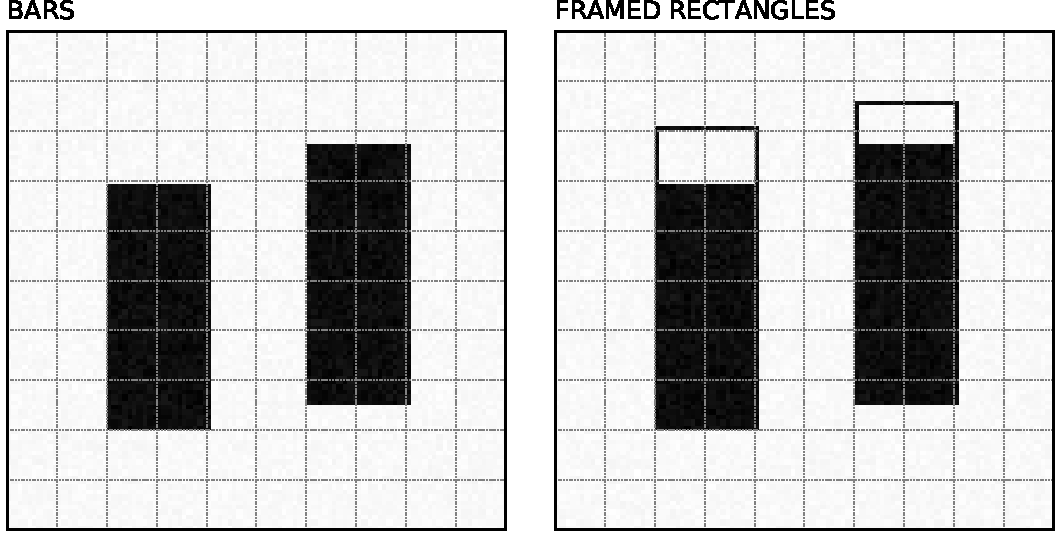
\includegraphics[width=\linewidth]{figure12_overview}
  \caption{\textbf{Bars and Framed Rectangles Experiment.} Cleveland and McGill introduce the bars and framed rectangles experiment which measures the perceptual task of judging position along non-aligned scales. For humans, it is easier to decide which of two bars represent a larger height if a scale is introduced by adding framed rectangles (right). In this case, the right bar is heigher as visible with less free space when adding the frame. We evaluate whether such a visual aid also helps machines to perceive visually encoded quantities.}
	\label{fig:bars_and_framed_rectangles_experiment}
\end{figure}

\subsection{Weber-Fechner's Law}

As identified by Cleveland and McGill, the bar and framed rectangle experiment is closely related to Weber's law. This psychophysics law states that perceivable difference within a distribution is proportional to the initial size of the distribution. Weber's law goes hand-in-hand with Fechner's law. We conduct an additional experiment based on the original illustrations of the Weber-Fechner law to investigate whether this law can be applied to computational perception of our classifiers (Fig.~\ref{fig:webers_law}).

\begin{figure}[t]
	  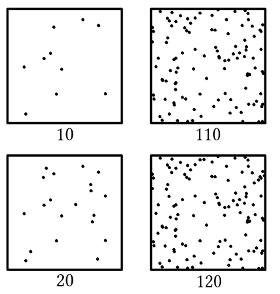
\includegraphics[width=\linewidth]{webers_law}
  \caption{\textbf{Weber-Fechner Law.} The Weber-Fechner law states that the perceivable differences within a distribution is proportional to the initial size of the distribution. The lower square contains 10 more dots than the upper one on both sides. However, the difference is easily perceivable on the left while the squares on the right almost look the same. We generate rasterized visualizations similar to this setup and evaluate our classifiers.}
	\label{fig:webers_law}
\end{figure}

\section{Results and Discussion}

\subsection{Elementary Perceptual Tasks}

some are good and some are bad.. why?

\begin{figure*}[h]
	  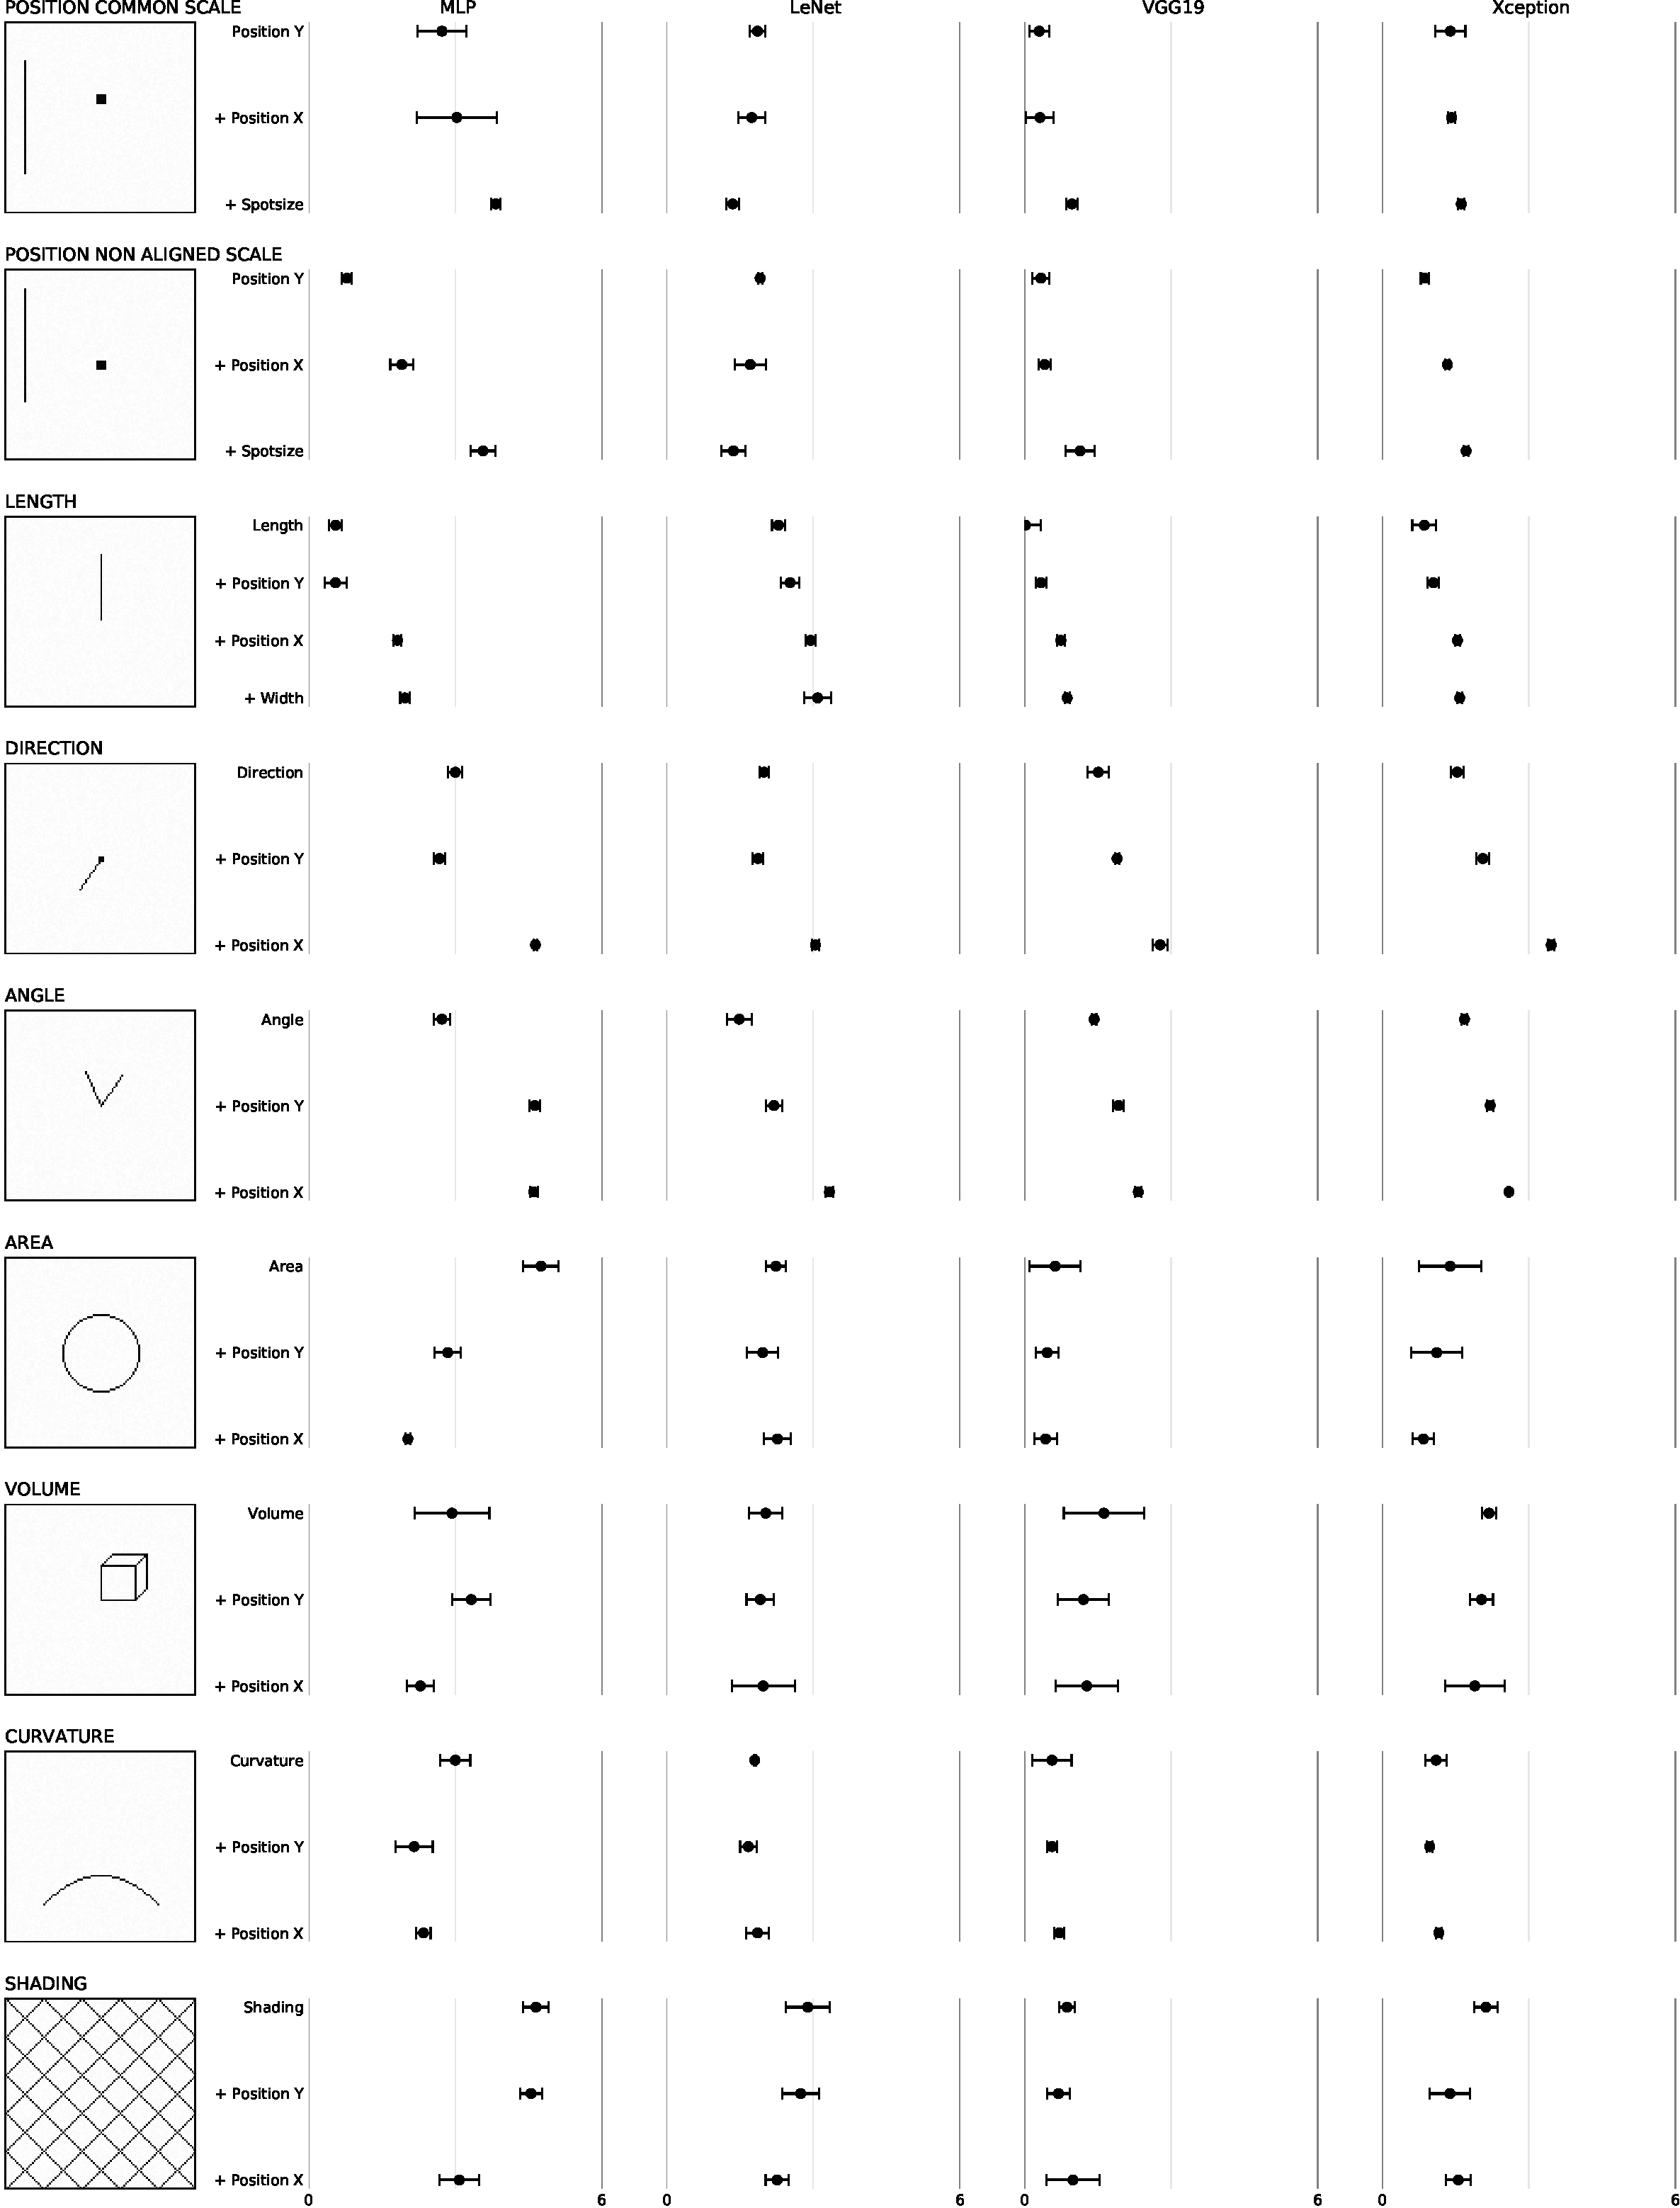
\includegraphics[width=\linewidth]{figure1.pdf}
  \caption{\textbf{Computational results of Elementary Perceptual Tasks experiment.} Log absolute error means and 95\% confidence intervals for computed perception of different classifiers on the \emph{elementary perceptual tasks} introduced by Cleveland and McGill 1984~\cite{cleveland_mcgill}. We test the performance of a Multi-layer Perceptron (MLP), the LeNet Convolutional Neural Network, as well as feature generation using the VGG19 and Xception networks trained on ImageNet.}
	\label{fig:figure1_results}
\end{figure*}

\textbf{Computational Perception Ranking.}

Cleveland McGills Ranking - can we observe something similar?

\begin{enumerate}
	\item Position along a common scale e.g. scatter plot
	\item Position on identical but nonaligned scales e.g. multiple scatter plots
	\item Length e.g. bar chart
	\item Angle \& Slope (tie) e.g. pie chart
	\item Area e.g. bubbles
	\item Volume, density, and color saturation (tie) e.g. heatmap
	\item Color hue e.g. newsmap
\end{enumerate}

\noindent{\textbf{Cross-classifier variability.}}

Can a neural network generalize on simple perceptual tasks?

\subsection{Position-Angle Experiment}

Bar charts are more accurate (Fig.~\ref{fig:figure3_mlae}) and networks converge faster (Fig.~\ref{fig:figure3_val_loss}). This is great.

\begin{figure}[t]
	  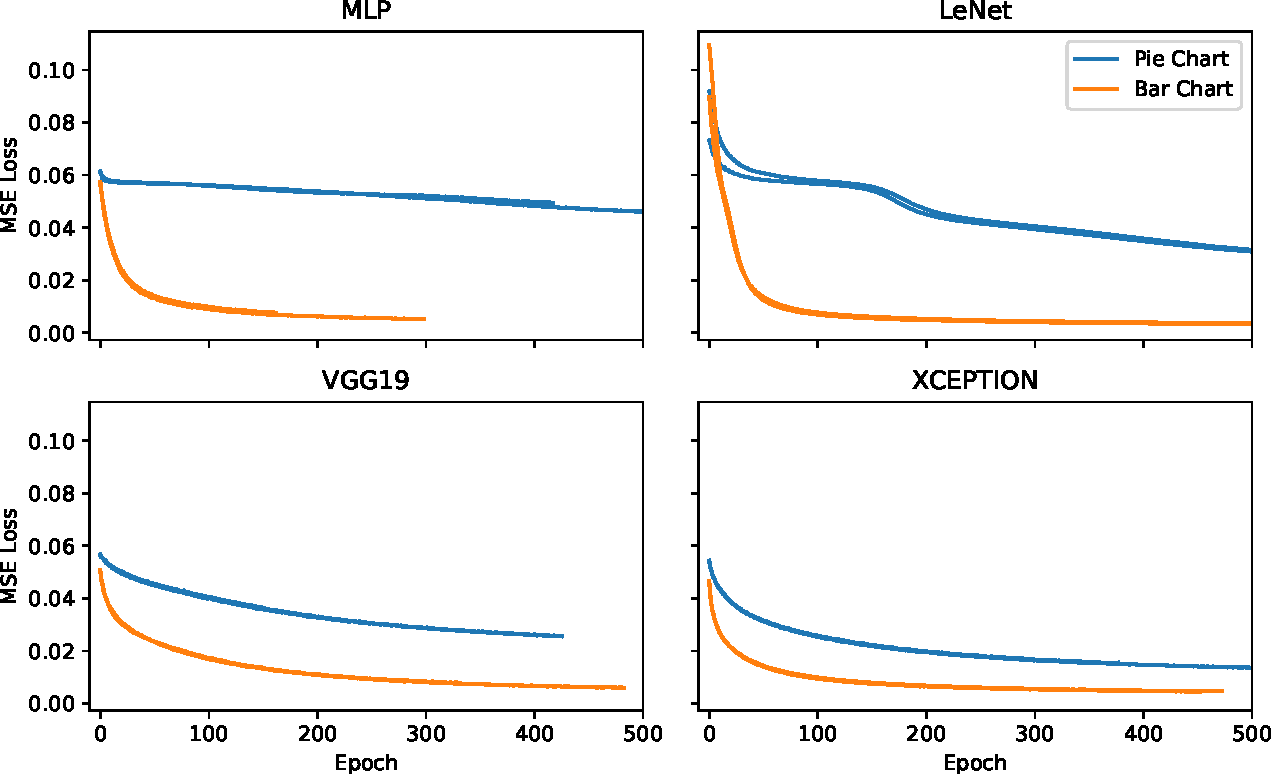
\includegraphics[width=\linewidth]{figure3_val_loss.pdf}
  \caption{\textbf{Classifier Efficiency of the Position-Angle experiment.} Mean Square Error (MSE) loss for the \emph{position-angle experiment} as described by Cleveland and McGill~\cite{cleveland_mcgill} which compares the visualization of pie charts and bar charts. We report the MSE measure for both encodings of four different classifier on previously unseen validation data.}
	\label{fig:figure3_val_loss}
\end{figure}

\begin{figure*}[t]
	  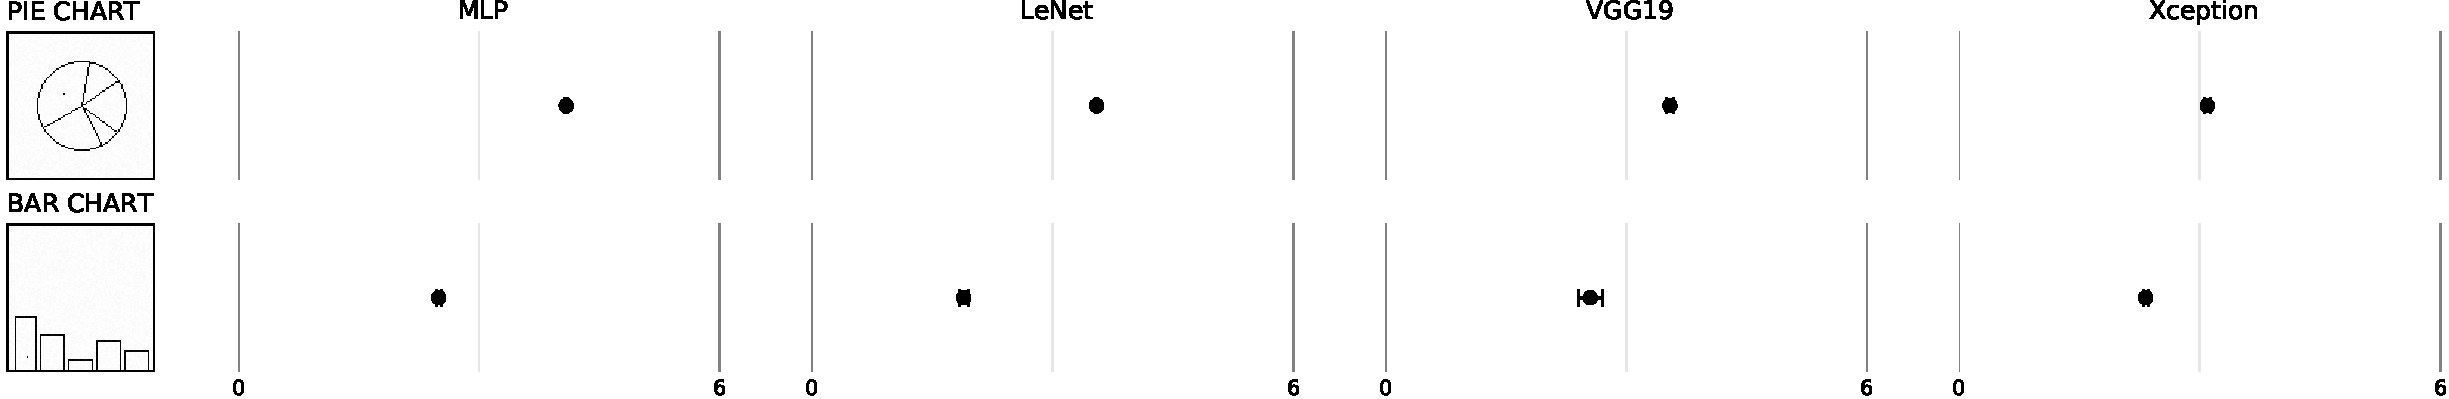
\includegraphics[width=\linewidth]{figure3_mlae.pdf}
  \caption{\textbf{Computational results of the Position-Angle experiment.} Log absolute error means and 95\% confidence intervals for the \emph{position-angle experiment} as described by Cleveland and McGill~\cite{cleveland_mcgill}. We test the performance of a Multi-layer Perceptron (MLP), the LeNet Convolutional Neural Network, as well as feature generation using the VGG19 and Xception networks trained on ImageNet.}
	\label{fig:figure3_mlae}
\end{figure*}

\subsection{Position-Length Experiment}

We have nothing yet here...


\subsection{Bars and Framed Rectangles Experiment}

First run indicates that framed rectangles perform better but we dont really know it yet.

\begin{figure}[t]
	  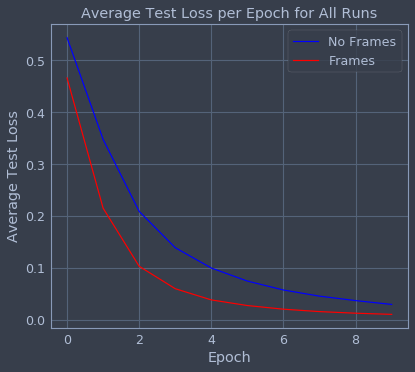
\includegraphics[width=\linewidth]{figure12_val_loss.png}
  \caption{\textbf{Classifier Efficiency of the Bars and Framed Rectangles experiment.} Categorical Cross-Entropy loss for the \emph{bars and framed rectangles experiment} as described by Cleveland and McGill~\cite{cleveland_mcgill}. The frame around the bars adds an additional visual cue enables faster network convergence. This is not yet reproducible!}
	\label{fig:figure12_val_loss}
\end{figure}


\section{Conclusions}

Future work: allow insights for infovis for machines


%% if specified like this the section will be committed in review mode
%\acknowledgments{
%The authors wish to thank A, B, and C. This work was supported in part by
%a grant from XYZ (\# 12345-67890).}

%\bibliographystyle{abbrv}
\bibliographystyle{abbrv-doi}
%\bibliographystyle{abbrv-doi-narrow}
%\bibliographystyle{abbrv-doi-hyperref}
%\bibliographystyle{abbrv-doi-hyperref-narrow}

\bibliography{paper.bib}
\end{document}

